\documentclass{article}
% Package to manage page layout
\usepackage[margin=1.5cm, includefoot, footskip=30pt]{geometry}

\setlength\parindent{0pt}
\setlength{\parskip}{1em}

%%%%%%%PACKAGES HERE%%%%%%%
\usepackage{amsmath}
\usepackage{hyperref}
\usepackage{standalone}
\usepackage{subcaption}
\usepackage{tikz}
\usetikzlibrary{er,positioning, calc}
%%%%%%%%%%%%%%%%%%%%%%%%%%%
\title{Literature review paper for the iterated prisoner's dilemma.}
\author{Nikoleta E. Glynatsi}
\date{2016}

\begin{document}

\maketitle

\section{Introduction}\label{section:introduction}

The emergence of cooperation is a topic of continuing and public interest
for social, biological and ecological sciences. The prisoner's dilemma is a 
fundamental game commonly used in the evolution of altruistic
behaviour.

The prisoner's dilemma is a two players no-cooperative game where the decisions
of the players are made simultaneously and independently. Both players can
choose between cooperation (\textbf{C}) and defection (\textbf{D}).

The fitness of each player is influenced by its own behaviour, and the behaviour
of the opponent. If both players choose to cooperate, both do better
than if both defected. A player has the temptation to deviate, cause if one
player were to defect while the other cooperates, the defector receives
more than if both had cooperated. The reward for mutual cooperation is \(R\)
units, for a mutual defection they receive \(P\), and for cooperation-defection,
the cooperator receives \(S\) where the defector receives \(T\).

Thus, the game's payoff are  defined by,

\begin{equation} \label{eq:the_pd_payoffs}
	\begin{pmatrix} 
	R & S \\ T & P
	\end{pmatrix},
\end{equation}

where,  \(T > R > P > S \) and \(2R > T + S.\) are the conditions for the dilemma
to exist. Due to rational behaviour and the knowledge that an individual is tempted 
to defect, the game's equilibrium lies at a mutual defection and both players 
receive a \(P\) payoff. Thus, the unbeatable strategy if the prisoner's dilemma 
is \textbf{D}.

Though the one shot game illustrate how  players will not trust their opponents
and  will act selfishly, choosing defection, greater insights can be achieved by 
studying the game in a manner where the prior outcomes matters. The 
repeated form is called the iterated prisoner's dilemma, and it will be discussed
later on how, it was proven to leave more room for cooperation to emerge. 

The origin of the prisoner's dilemma go back to 1950 in early experiments 
conducted in RAND~\cite{Flood1958} to test the applicability of games
described by~\cite{VonNeumann1944}.  In~\cite{Flood1958} they introduced 
a two player non-cooperative game but the story behind the game was
given later the same year. A. W. Tucker, who was John Nash's supervisor, in 
his attempt to tell a story during one of his talks gave the background story of 
the prisoner's dilemma as we know it today~\cite{Tucker1983}. 

In the following section several milestones on the research of the prisoner's
dilemma are presented and discussed.  Figure~\ref{fig:timeline} illustrates
a timeline generated using the open source library discussed in 
Section~\ref{section:analysis}. This illustrates that the prisoner's dilemma has
been under continuous research since it's origins. Several insights and applications
have been offered in research by the game, these will be discussed in the 
following sections.

\begin{figure}[!htbp]
    \centering
    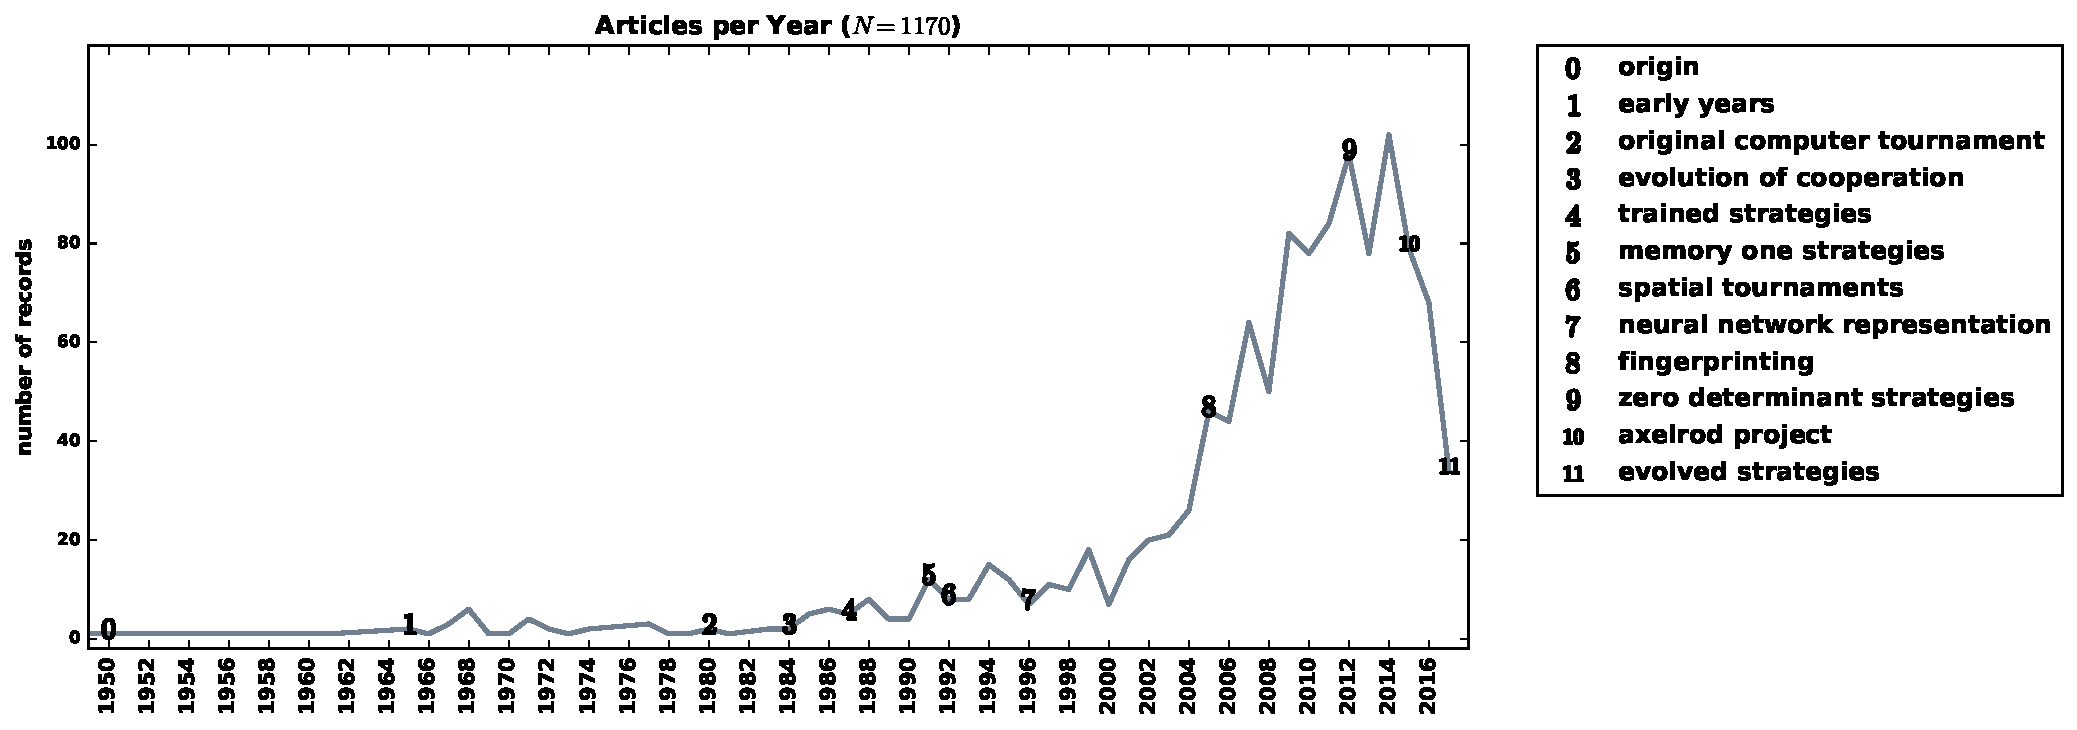
\includegraphics[width=\textwidth]{assets/images/timeline.pdf}
    \label{fig:timeline}
    \caption{A timeline highlighting the milestones of the prisoner's dilemma.}
\end{figure}

\section{Timeline}\label{section:timeline}

\subsection{Early Years}
The study of the prisoner's dilemma attracted people from various field.
An important figure within the field is professor Anatol Rapoport, a mathematical
psychologist focused on war and peacekeeping.  
In his early work~\cite{rapoport1965} he conducted experiments using humans
to simulate the interactions of prisoner's dilemma game. Human experiments
have not been used only by Prof Rapoport, instead it was a common way of
studying the game~\cite{Evans1966, Gallo1968, Lutzker1961, Mack1971, 
Sensenig1972} and it still being used to date. %REF

These early experiments explored the conditions under which altruist behaviour
emerges. Researchers were in search of an unbeatable strategy to play the game. 
Inspired by the work of Rapoport and the idea that AI was trained to play the 
game of chess~\cite{axelrod2012}, the political scientist R. Axelrod performed
the first ever computer tournament, known to the author, of the iterated 
prisoner's dilemma~\cite{Axelrod1981}.

\subsection{Reciprocal Period}\label{subsection:reciprocal}
In 1980~\cite{axelrod1980a} a computer tournament of the iterated prisoner's 
dilemma took place with 14 participants. The tournament was of a round robin 
topology where each strategy played against all the opponents, itself and the 
Random strategy (a  strategy that chooses between \textbf{C} and \textbf{D}
randomly). Each
participant knew the exact length of the matches and had access to full history
of each match.  The payoffs values of (\ref{eq:the_pd_payoffs}) used by Axelrod
were the following, \(R=3, P=1, T=5\) and \(S=0\).  These values are the most 
common used in literature and assume that they are being used in the works 
referenced from now on unless is stated otherwise. The winner of the tournament 
was determined by the total average score and not by the number of matches 
wins. The strategy that was announced the winner was submitted by Prof. 
Rapoport and was called called Tit For Tat.

Tit for Tat, was a strategy that always cooperated on the first round and then
mimics the opponent's previous move. his is illustrated diagrammatically in 
Figure~\ref{fig:tit_for_tat_diagram}. To further test the robustness of the 
results a second tournament was performed later with a total of 63 strategies
\cite{axelrod1980b}. All the opponents knew the results of the previous 
tournament by this time the number of turns was not specified. Instead
a probabilistic ending tournament was used. Each match has probability of 
ending after each move. This is also refereed as `shadow of the future'
is some other works~\cite{axelrod1988}. The winner of the second tournament
was once again the strategy Tit For Tat. Tit for tat was an example of how reciprocity
behaviour allows for cooperation to emerge in the iterated game.

\begin{figure}[!hbtp]
    \centering
    \includestandalone[height=.3\textheight]{./assets/tex/tit_for_tat_diagram}
    \caption{Diagrammatic representation of Tit for Tat.}
    \label{fig:tit_for_tat_diagram}
\end{figure}

According to Axelrod, the secrets behind the strategy's success have been
1) that it start of by cooperating 2) it would forgive it's opponent after a
defection 3) after opponents identified that they were playing Tit for Tat choose 
to cooperate for the rest of the game. 

In~\cite{Axelrod1981}, the strategies set of second tournament was used
to perform a ecological kind of tournament. The 63 strategies interact generation
after generation to a round robin competition where their frequencies is proportional
to their payoff in the previous round. Results showed that in a homogeneous
population of Tit for Tat invasion by mutant strategies was not successful. 
The success of Tit For Tat was very soon  known world wide and several researcher
focused their work on the strategy ever since.%REF

\subsection{Stochastic Environments}
But success often comes with criticism. Axelrod's tournaments assumed that
each player has perfect information of the opponent's actions. In real life 
situation this is not always the case. Colleagues interactions 
often suffer from measures of uncertainty. In the original tournaments
there was no possibility of misimplementation or misunderstanding. These
stochastic variations are often called \textbf{noise} and \textbf{misperception}.

Noise is the concept of flipping ones moved based on a probability. On the
contrary, misperception is the probability that the opponent’s current move is 
flipped before being recorded. Noise will flip a player’s action it will be recorded 
correctly in the history where mis perception will not have an effect on the player 
move but it will be recorded wrong~\cite{Hoffmann1998}.The performance of
Tit for Tat was proven to suffer from such stochasticity in the tournament 
environment, especially against itself~\cite{Bendor1991,Godfray1992, 
Molander1985, Nowak1992}.

An interesting result was introduced by~\cite{Molander1985}.  If two players are
both using the Tit for Tat strategy, both players would get the same average
payoffs as two interacting Random players with \(p=0.5\). 
In~\cite{Nowak1992}, they used evolutionary dynamics and showed that to cope
with noise a more generous version of Tit for Tat is needed.  

\subsection{Era of Strategies}

Following the pioneer work of computer tournaments many researchers have sought to
understand which strategies are dominant when playing the repeated prisoner's
dilemma. These strategies can be anything, from deterministic to complex. The 
can make  use of the history of the game, the length or nothing at all. The size 
of history a strategy takes into account is refereed to as memory size of the
strategy. %REF

The two most common deterministic strategies used in various works are 
\textbf{All Defector} and \textbf{All Cooperator}. Both strategies have been 
introduced in~\cite{Axelrod1981}. All Defector defects in each turn, compared
to All Cooperator which is a strategy that always cooperates. 

In~\cite{Nowak1992}, the space of re-active strategies was explored and the 
strategy that stand out  was a re-active strategy known as \textbf{Generous Tit for Tat}. 
Reactive strategies are denoted by the probabilities to cooperate after a
\textbf{C} and a \textbf{D} of the opponent. Thus, a reactive strategy
only considers the previous turn of the opponent.

Reactive strategies are a subset of memory one strategies introduced in 1989
\cite{nowak1989}. Memory one strategies, are a set of strategies that 
consider only the last turn of the game to decide on the next action~\cite{Nowak1990}.
They are represented by the four conditional probabilities \(p_1, p_2, p_3\) and
\(p_4\) to cooperate after \(CC, CD, DC\) and \(DD\) respectively
(the four possible states a player can be in if only the last turn of the game was
to be considered). Reactive strategies are just a constrained version where 
\(p_1=p_3\) and \(p_2=p_1\). 

% A few examples of strategies that have been discussed can be 
% in their reactive representation are the following,

% \begin{itemize}
% 	\item Tit for Tat - \((p_1=1, p_2=0)\),
% 	\item Generous Tit for Tat - \((p_1=1, p_2=\frac{1}{3})\).
% \end{itemize}

The first action of the strategy (when the history does not exist yet) is assumed
to be \textbf{C} unless is stated otherwise. For example, a strategy called
\textbf{Suspicious Tit for Tat}, studied in~\cite{Nowak1992}, has the same representation
as Tit for Tat but plays \textbf{D} in the first round.

In 1993~\cite{Nowak1993}, an interesting memory-one  strategy with the 
tolerance of Generous Tit for Tat but the capability of resisting and invading
an all-out cooperators population was introduced. The strategy is called \textbf{Pavlov},
and is based on the fundamental behavioural mechanism win-stay, lose-shift.
The strategy starts off with a \textbf{C}, then Pavlov will repeat it's last 
move it was awarder with by \(R\) or \(T\) but will shift if punished by \(P\) or \(S\).

Several other strategies were introduced as more generous versions and 
described as more dominant than Tit for Tat. These include, \textbf{Contrite Tit for Tat}
\cite{Wu1995} and \textbf{Adaptive Tit for Tat}~\cite{tzafestas-2000a}. On the
other hand, defector variants have also been studied~\cite{Hilde2013}.
\textbf{Anti Tit for Tat}, is a strategy that plays the opposite of the opponents
previous move. Another limitation of the strategy was discussed in~\cite{Wolfgang2006}.
Tit for Tat was proven to hit a deadlock. Deadlock meaning a loop between 
cooperation and defection. \textbf{Omega Tit For Tat} was introduced and was
a strategy capable of avoiding the deadlock~\cite{Wolfgang2006}.

Other strategies that made an impact have been \textbf{Gradual}~\cite{Beaufils1997}
and \textbf{Handshake}~\cite{Robson1989} presented in 1997 and 1989 respectively.
Gradual starts off by cooperating, then after the first defection of the other player, 
it defects one time and cooperates twice. After the second defection of the opponent,
it defects two times and cooperates twice. After the n th defection it reacts with 
\(n\) consecutive defections and then two cooperations. 
Handshake is a strategy that starts with cooperation, defection. If the opponent plays in
a similar way then it will cooperate forever, otherwise it will defect forever.

In 2011~\cite{Li2011} performed their own tournament where several interesting
strategies made an appearance. 

\begin{itemize}
    \item \textbf{Periodic player CCD}, plays \textbf{C}, \textbf{C}, \textbf{D} 
    periodically. Note that variations of a period player also make appearance
    in the article but will not be listed here.
    \item \textbf{Prober}, starts with the pattern \textbf{D}, \textbf{C}, \textbf{C}
     and then defects if the opponent has cooperated in the second and third move;
     otherwise, it play as Tit for Tat.
    \item \textbf{Reverse Pavlov}, a strategy that does the reverse of Pavlov.
\end{itemize}

In earlier work the same author introduced a strategy called \textbf{APavlov},
which stands for adaptive Pavlov~\cite{Li2007}. The strategy attempts to 
classify the opponent as one of the following strategies, All Cooperator, 
All Defector, Pavlov, Random or \textbf{PavlovD}. PavlovD, is just Pavlov
but it starts the game with a \textbf{D}. Once Adaptive Pavlov has classified
the opponent plays to maximize it's payoff.

In~\cite{Ashlock2006b} two new strategies are presented. These strategies have
been trained using a finite state machine representation. They are called, 
\textbf{Fortress3} and \textbf{Fortress4}. Figure~\ref{fig:fortress3_and_4}
illustrates their diagrammatic representation.

\begin{figure}[!hbtp]
\centering
    \begin{subfigure}{.3\textwidth}
        \includestandalone[width=\textwidth]{assets/tex/fortress_3}    
    \end{subfigure}
    \begin{subfigure}{.3\textwidth}\centering
        \includestandalone[width=\textwidth]{assets/tex/fortress_4} 
     \end{subfigure}
     \caption{Representations of Fortress 3 and Fortress 4. Transition arrows are 
     labelled \textit{O/P} where \textit{O} is the opponent’s last action and \textit{P}
     is the player’s response. Note that the strategy’s first move, enters state 1, 
     is defection for both strategies.}
     \label{fig:fortress3_and_4}
\end{figure}

Finite state machines are a common mean of representing iterated prisoner's
dilemma strategies~\cite{Miller1996, Rubinstein1986}. Other representation
methods include lookup tables~\cite{Axelrod1987, Lindgren1994} and 
artificial neural networks~\cite{Fogel1996, Lee2015}.
A summary of several representation of the iterated prisoner's dilemma strategies
is given in~\cite{Knight2017}, the different representations are referred to as
archetypes. 

% A memory one representation of strategies are the following, 

% \begin{itemize}
% 	\item Tit for Tat - \((p_1=1, p_2=0, p_3=1, p_4=0)\) or for simplicity 
% 	\((1, 0, 1, 0)\),
% 	\item Pavlov - \((1, 0, 0, 1)\).
% \end{itemize}

% A diagrammatic representation of Pavlov is given in Figure~\ref{fig:pavlov_fsm},
% using a 2 state finite machines.  Finite state machines are a common mean of representing
% iterated prisoner's dilemma strategies~\cite{Rubinstein1986, Miller1996}. 

% \begin{figure}[!hbtp]
%     \centering
%     \includestandalone[width=.4\textwidth]{./assets/tex/pavlov}
%     \caption{Diagrammatic representation of Pavlov using a finite state machine.}
%     \label{fig:pavlov_fsm}
% \end{figure}

% Note that the transition arrows are labeled \textit{O/P} where \textit{O} is the 
% opponent’s last action and \textit{P} is the player’s response. 
% The initial move of the strategy, enters state 1, is \textbf{C}. An example,
% of how several strategies can be represented in a similar manner is given
% by Figure~\ref{fig:tit_for_tat_fsm}, illustrating the strategy Tit for Tat.

% \begin{figure}[!hbtp]
%     \centering
%     \includestandalone[width=.2\textwidth]{./assets/tex/tit_for_tat_fsm}
%     \caption{Diagrammatic representation of Tit for Tat using a finite state machine.}
%     \label{fig:tit_for_tat_fsm}
% \end{figure}

\subsection{Strategies Stability}

A strategy's robustness is tested through out the interactions and the performance
of the strategy in a tournament against other strategies. Is the overall
success of a strategy based only on it's performance in a round robin tournament,
or should the strategy's performances be checked through other ways as well.

Following his initial tournaments Axelrod performed an `ecological' tournament
in 1981~\cite{Axelrod1981}.  The ability of strategies to be favoured under
natural selection and their ability to withstand invasion from other strategies
soon became an new measure of performance. 

The ecological approach is based on the payoff matrix of the tournament.  The
highest performing strategies are adapted by lower scoring individuals
within a fixed population. Over time a strategy takes over the population.

\begin{figure}[!hbtp]
    \centering
    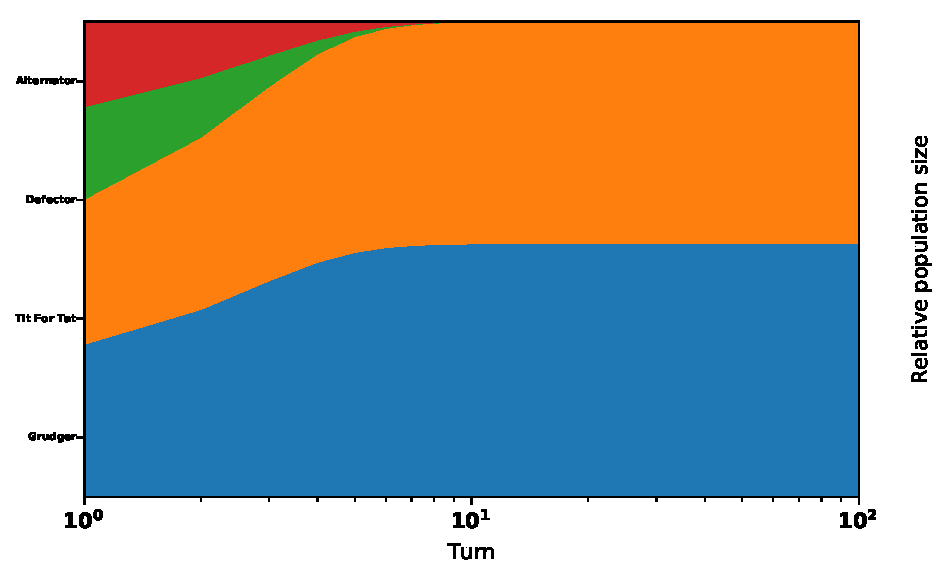
\includegraphics[width=.6\textwidth]{./assets/images/ecological.pdf}
    \caption{System evolving over time based on natural selection using
    \cite{axelrodproject}.}
    \label{fig:ecological.tournament}
\end{figure}

Axelrod and his reciprocal claims were put on the test once again. 
The results of~\cite{Boyd1987} argued that no pure strategy is evolutionary
stable in the iterated prisoner's dilemma. This was not proven analytically, instead
a series of examples using strategies such as Tit for Tat, Suspicious
Tit for Tat and All Defector where explored; a very constrained set of strategies.

The results were questioned by~\cite{May1987}, they stated that much was 
still no fully explored and more research had to be put into the results. 
Another attempt to explore stability of strategies in the prisoner's dilemma
was done in~\cite{Boyd1989}. This time exploring the results in a noisy
environment, but similarly a analytical prove was not given.

An extension to the natural selection was introduced in the 1992~\cite{Nowak1992},
recommending a different type of topology. A population of two deterministic
strategies, AllD and AllC, are placed on a a two dimensional square array
where the individuals can now interact only with the immediate neighbour. 
In this work it was proven that cooperation will emerge if individuals interact
in neighbourhoods. The new topology has been called every since, spatial 
topology in the literature. %REF

\textit{Nowak and moran process.} 

\subsection{Software} 

Due the nature of the research regarding the iterated prisoner's dilemma
several software packages have been created in order to simulate the 
computer tournaments.

The earliest source code that can be found, to the authors knowledge, is that
of Axelrod's second tournament~\cite{axelrod1980b}.  The code has been 
written by Axelrod and several other contributors in the programming 
language Fortran~\cite{fortan_code}. The site specifically says that the course 
code of the initial tournament is not available. 

Another  piece of software includes a library called PRISON. PRISON is 
is written in the programming language Java and it has been used by it's authors
in several publications. The project includes a good number of strategies from
the literature but unfortunately the last update of the project dates back in 2004.

More recent projects include~\cite{pd_trust, pd_game}. Note that~\cite{pd_trust}
is a user interface project that introduces several concept of the research.
Such as the iterated game, computer tournaments and evolutionary
dynamics. The list of strategies included is very limited. On the other hand,
\cite{pd_game} offers a bigger collection of strategies. The users are also
able to introduce the concept of noise in their tournaments. Even so, 
it remains a user interface project and makes it constrained for a research tool. 

In 2015 an open source library, called the Axelrod project was introduced
\cite{axelrodproject}. The project is written in the programming language 
Python, it is accessible and open source. To date the list of strategies implemented
within the library exceed the 200. The project has been used in several
publications including~\cite{Knight2017} and a paper describing it and
it's capabilities was published in 2016~\cite{Knight2016}.

Software has a crucial role in research. Well written and maintained softwares
allows the reproducibility of prior work and can accelerate findings withing the
field. The field of the iterated prisoner's dilemma has suffered the consequences
of poor research software. As stated above the source code of the initial
computer tournament is not retrievable. Several of the strategies that competed
in the tournament are not given a full explanation of how the decided on their
next move. 

In~\cite{Rapoport2015}, the authors claim that they have managed to 
re-run the first tournament that Axelrod performed. They tried to push his work
further by altering aspects such as, the format of the tournament, the objective
and the population. One of the authors claimed to have been a contributor
to the first tournaments, which would explain how it was managed to reproduce
the tournament.

A more recent work discuss the issues raised in here on the importance 
of research software and questions several results of the initial tournaments.%REf

\subsection{Ecological Applications}

The reciprocal period of the prisoner's dilemma spread the knowledge of the
game not only worldwide but also across different scientific principles. The
study of cooperation was once again a critical issue. The applications of
the game soon found their way to ecological studies, for example 
\cite{Milinski1987} conducted an experiment using sticklebacks to test
the robustness of the strategy Tit for Tat in the interactions of fish. Fish usually
travel in pairs and monitor their hunters to gain information on the enemy.
Other works that include applications to ecological settings have been those
of~\cite{Godfray1992, Wilkinson1984}. There the reciprocal food sharing
between vampire bats was studied.

\subsection{not sure yet}
In his works~\cite{axelrod1988} try to address the criticism by studying Tit for 
Tat in an evolutionary manner as well. It was shown that Tit For Tat does not 
perform as well in noisy and in environments with mis-perception, but there are 
variants of Tit for Tat that do.




\section{Analysis}\label{section:analysis}

\bibliographystyle{plain}
\bibliography{bibliography.bib}
\end{document}